\chapter{Results}
\chlab{results}

In the user studies, a lot of different types of data has been created. First, graphical representations of most observations from the user action log can be found in \appref{graphs}. In that same chapter, the outcomes of the \verb|SUS| and \verb|UMUX| questions that were asked in the questionnaire can also be found. \Appref{comments} contains all answers to the open questions, including general comments about the system, the preferred version and suggestions for improvement.

This chapter will contain the important and most interesting results obtained in the user studies. Each result will shortly be discussed, and further analysed in \chref{discussion}.


\section{Action log results}
\nlipsum

\subsection{Time required}
\nlipsum

\begin{figure}
\center
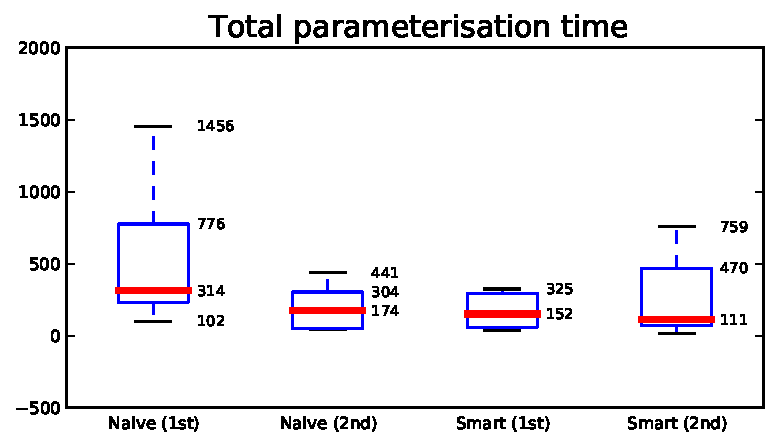
\includegraphics[width=.9\textwidth]{img/graphs/1a_02.pdf}
\caption{Total parameterisation time for the two versions in the two orders.}
\figlab{graph_time_1}
\end{figure}

\begin{figure}
\center
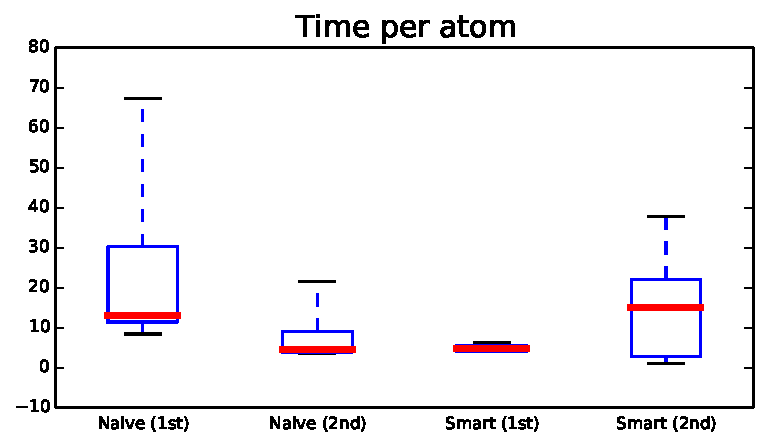
\includegraphics[width=.9\textwidth]{img/graphs/1a_03.pdf}
\caption{Average time per fragment for the two versions in the two orders.}
\figlab{graph_time_2}
\end{figure}

\begin{figure}
\center
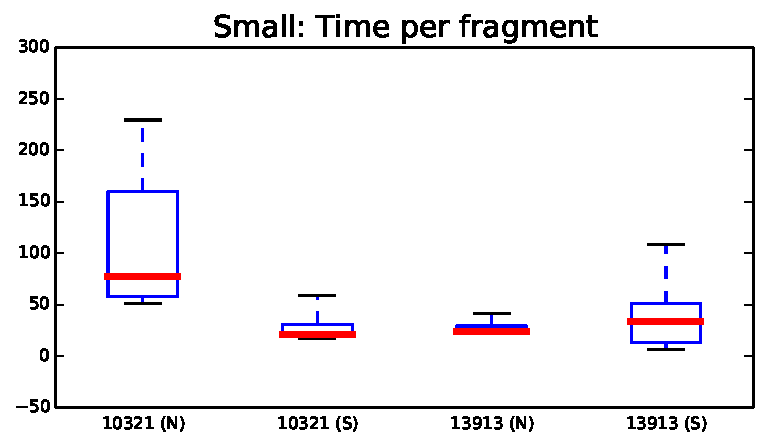
\includegraphics[width=.9\textwidth]{img/graphs/1b_03.pdf}
\caption{Average time per fragment for the smaller molecules in the two orders.}
\figlab{graph_time_3}
\end{figure}

\begin{figure}
\center
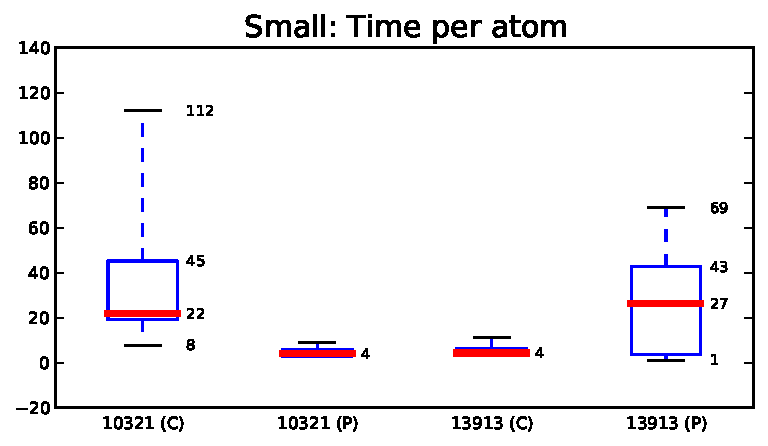
\includegraphics[width=.9\textwidth]{img/graphs/1c_03.pdf}
\caption{Average time per fragment for the larger molecules in the two orders.}
\figlab{graph_time_4}
\end{figure}

\subsection{Parameterisation rating}
\nlipsum

\begin{figure}
\center
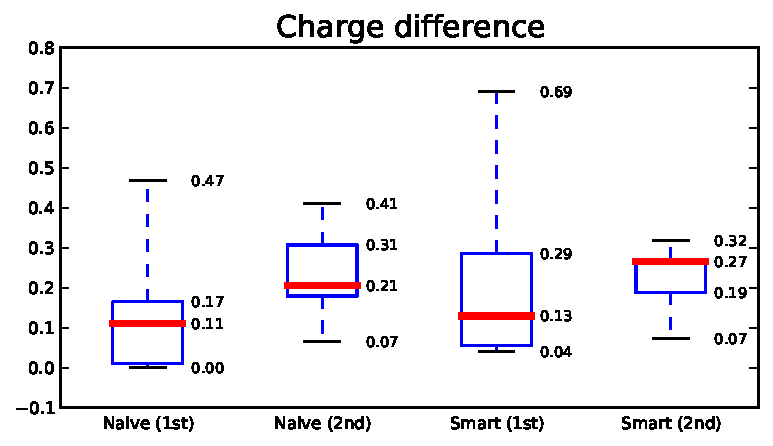
\includegraphics[width=.9\textwidth]{img/graphs/1a_00.pdf}
\caption{Total charge difference for the two versions in the two orders.}
\figlab{graph_rating_1}
\end{figure}

\begin{figure}
\center
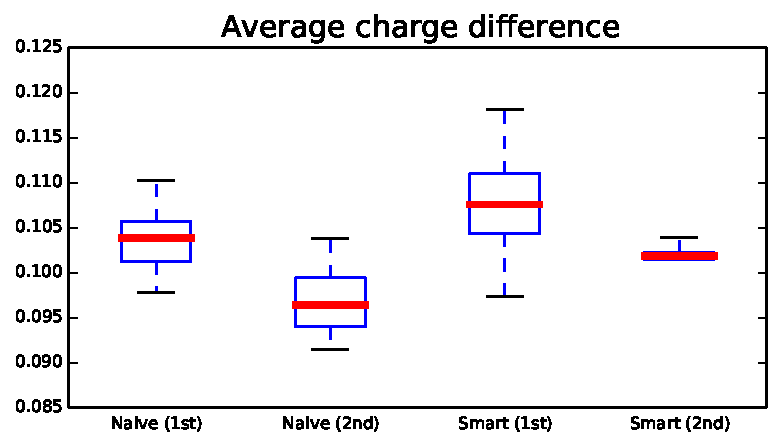
\includegraphics[width=.9\textwidth]{img/graphs/1a_01.pdf}
\caption{Average charge difference per atom for the two versions in the two orders.}
\figlab{graph_rating_2}
\end{figure}

\begin{figure}
\center
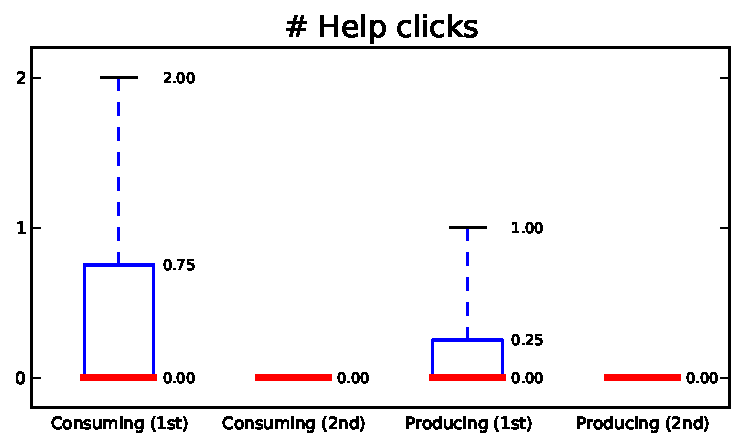
\includegraphics[width=.9\textwidth]{img/graphs/1b_01.pdf}
\caption{Average charge difference per atom for the smaller molecules in the two orders.}
\figlab{graph_rating_3}
\end{figure}

\begin{figure}
\center
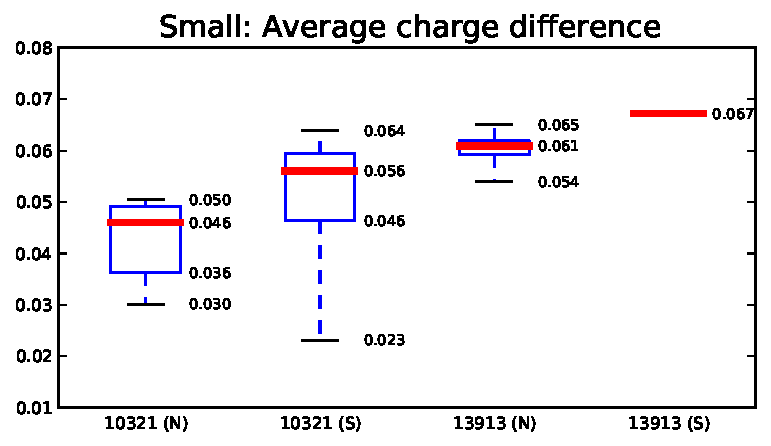
\includegraphics[width=.9\textwidth]{img/graphs/1c_01.pdf}
\caption{Average charge difference per atom for the larger molecules in the two orders.}
\figlab{graph_rating_4}
\end{figure}

\subsection{Other results}
\nlipsum

\subsubsection{Undo operations}
\nlipsum

\begin{figure}
\center
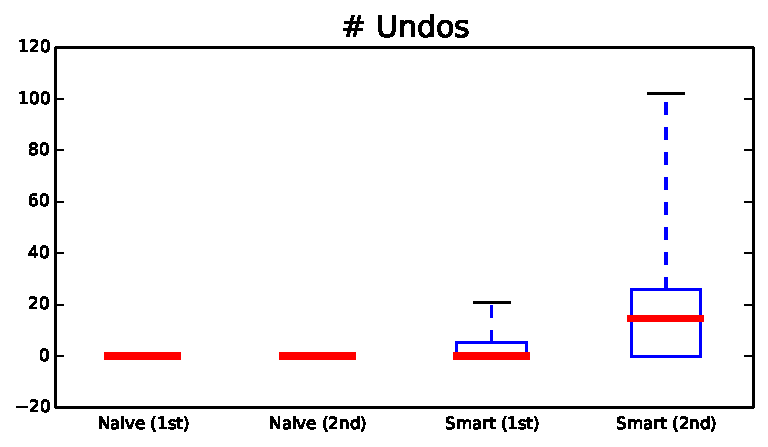
\includegraphics[width=.9\textwidth]{img/graphs/1a_10.pdf}
\caption{Number of undo actions for the two versions in the two orders.}
\figlab{graph_undo}
\end{figure}

\subsubsection{Clicks}
\nlipsum

\begin{figure}
\center
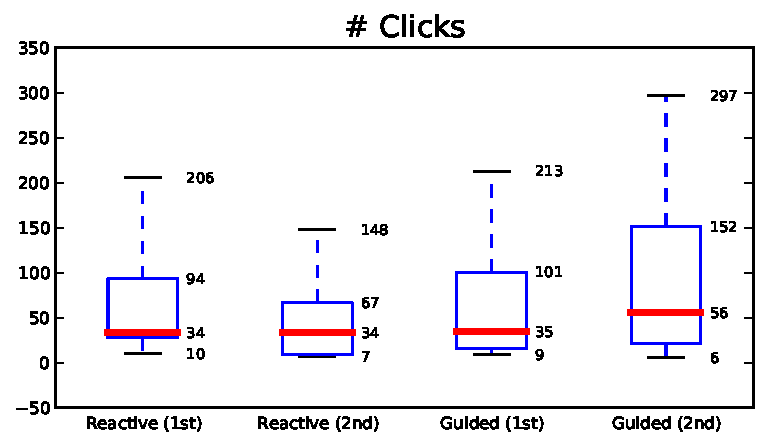
\includegraphics[width=.9\textwidth]{img/graphs/1a_04.pdf}
\caption{Total number of clicks for the two versions in the two orders.}
\figlab{graph_clicks}
\end{figure}

\subsubsection{Help}
\nlipsum

\begin{figure}
\center
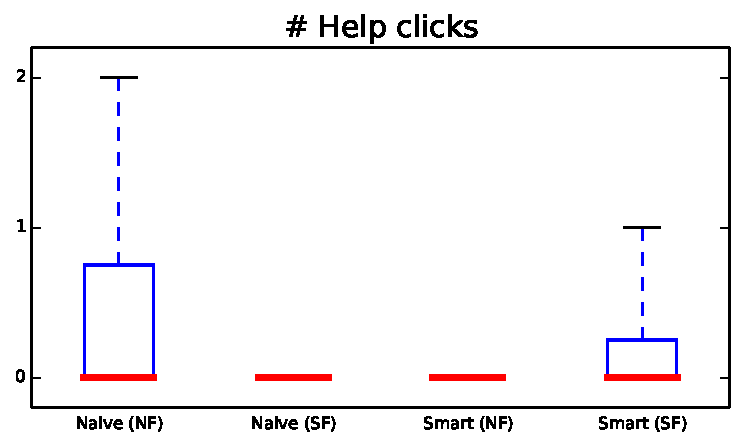
\includegraphics[width=.9\textwidth]{img/graphs/2_01.pdf}
\caption{Total number of clicks on the help button for the two versions in the two orders.}
\figlab{graph_help}
\end{figure}

\subsection{Correlations}
\nlipsum

\begin{figure}
\center
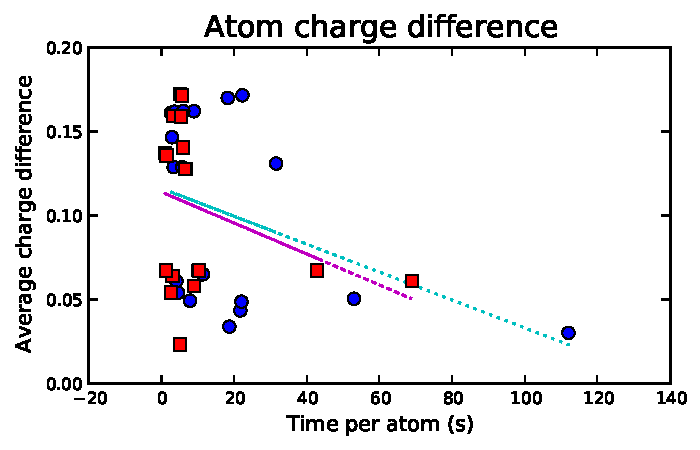
\includegraphics[width=.9\textwidth]{img/graphs/3a_00.pdf}
\caption{Average charge difference per atom in relation to the time used per fragment.}
\figlab{graph_correlation_1}
\end{figure}

\begin{figure}
\center
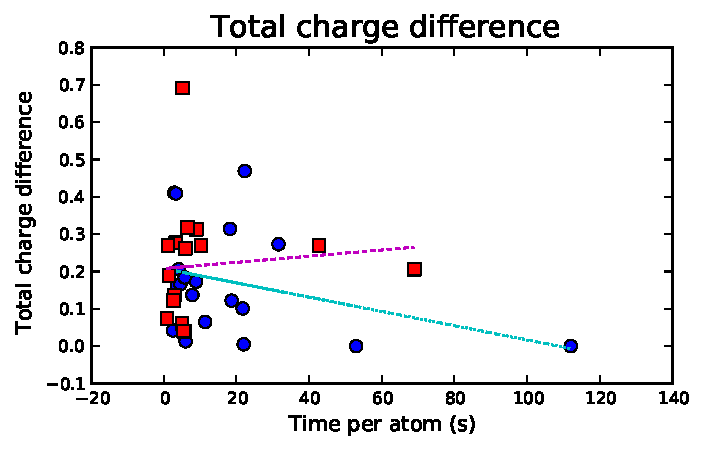
\includegraphics[width=.9\textwidth]{img/graphs/3a_01.pdf}
\caption{Average charge difference per atom in relation to the total time used.}
\figlab{graph_correlation_2}
\end{figure}

\begin{figure}
\center
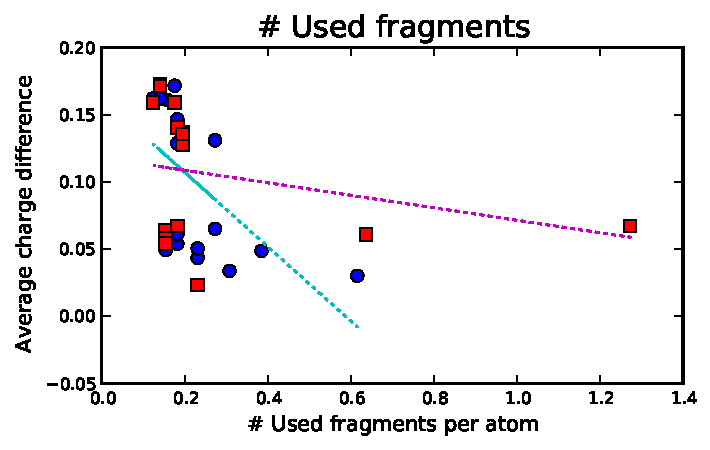
\includegraphics[width=.9\textwidth]{img/graphs/3a_02.pdf}
\caption{Average charge difference per atom in relation to the number of used fragments per atom.}
\figlab{graph_correlation_3}
\end{figure}

\begin{figure}
\center
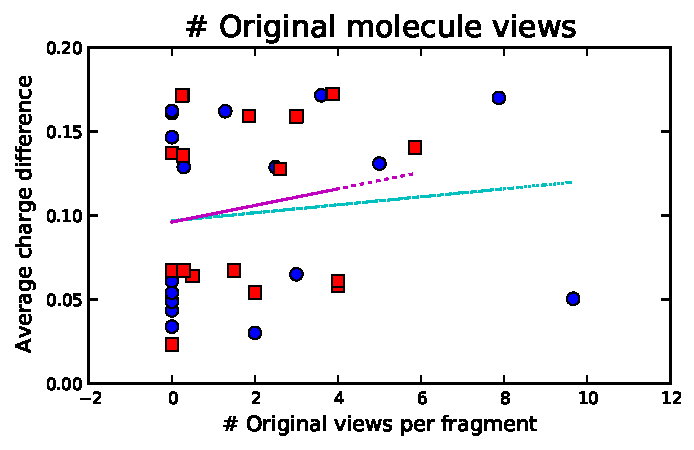
\includegraphics[width=.9\textwidth]{img/graphs/3a_03.pdf}
\caption{Average charge difference per atom in relation to the number of original molecule views per used fragment.}
\figlab{graph_correlation_4}
\end{figure}


\section{Questionnaire outcomes}
\nlipsum

\subsection{\texttt{SUS} / \texttt{UMUX} results}
\nlipsum

\begin{figure}
\center
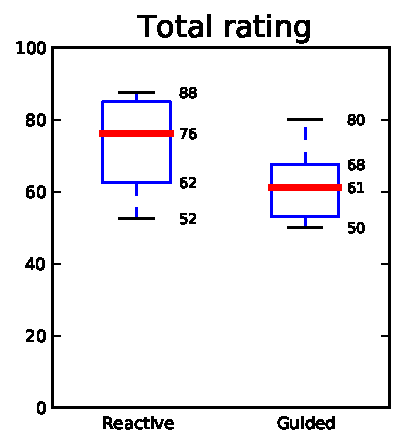
\includegraphics[width=.9\textwidth]{img/graphs/4a_10.pdf}
\caption{Average rating for the two versions.}
\figlab{graph_rating_1}
\end{figure}

\begin{figure}
\center
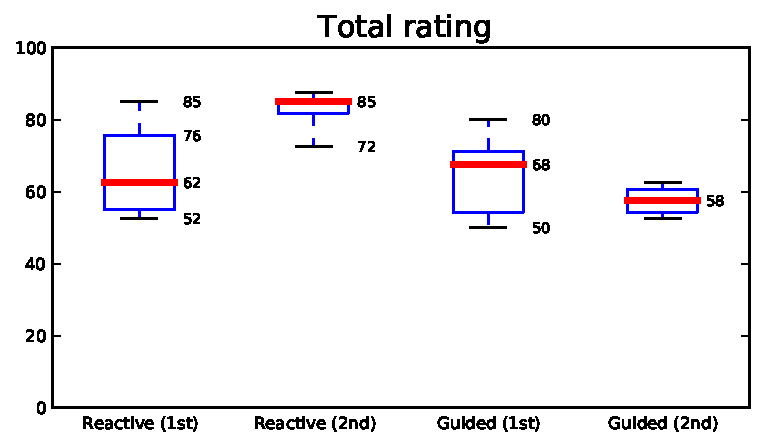
\includegraphics[width=.9\textwidth]{img/graphs/4b_10.pdf}
\caption{Average rating for the two versions in the two orders.}
\figlab{graph_rating_2}
\end{figure}

\begin{figure}
\center
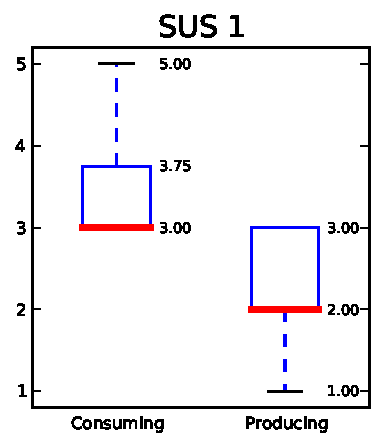
\includegraphics[width=.9\textwidth]{img/graphs/4a_00.pdf}
\caption{Rating of \texttt{SUS1} for the two versions.}
\figlab{graph_rating_3}
\end{figure}

\begin{figure}
\center
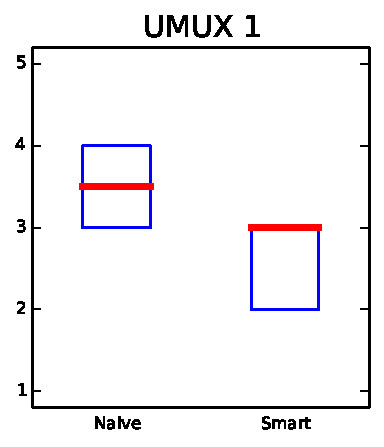
\includegraphics[width=.9\textwidth]{img/graphs/4a_01.pdf}
\caption{Rating of \texttt{UMUX1} for the two versions.}
\figlab{graph_rating_4}
\end{figure}

\begin{figure}
\center
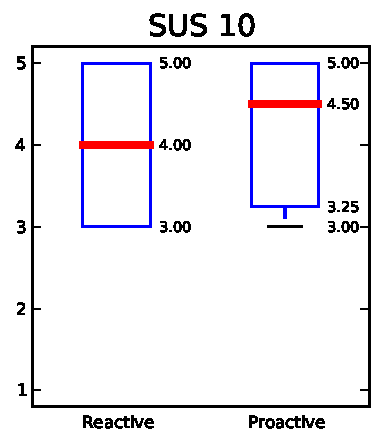
\includegraphics[width=.9\textwidth]{img/graphs/4a_09.pdf}
\caption{Rating of \texttt{SUS10} for the two versions.}
\figlab{graph_rating_5}
\end{figure}

\subsection{Comments}
\nlipsum
